\chapter{Methodology}
 Agile Project Development can be properly used to guarantee the whole success of the project. Therefore,  we used Agile methodology as described below.
\section{Agile methodology}
 Agile methodologies are used to develop software based on the concept of the iterative development process.It abandons the risk of spending months or years on a process that ultimately fails because of some small mistake in an early phase.\\
Inside Agile, scrum framework can be used to manage all the project through clickUp.
Scrum is an Agile-based project management framework where teams develop products in short project cycles called sprints. At the end of each sprint, we gather customer feedback and incorporate their suggestions before continuing our development process.\\
\begin{figure}[H]
    \centering
    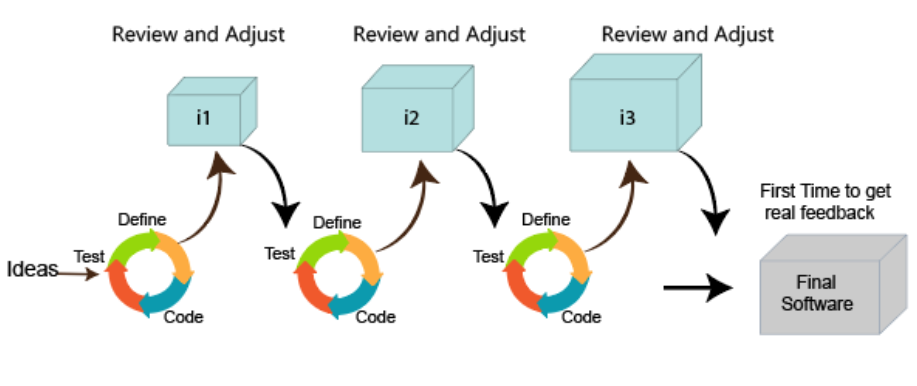
\includegraphics[width=1\textwidth]{img/chapter_4/agile.png}
    \caption{Agile methodology}
\end{figure}
\noindent
\subsection{Scrum Framework}
In the scrum method, we follow an incremental and iterative process to project management.
Here the project’s life cycle is split into smaller cycles of specific time periods (called sprints) that we tackle independently. Each sprint has a recommended duration of 2–4 weeks and will help us quickly develop our project and reach our deadlines on time.\\
After each sprint cycle is complete, we present the working software (called increment) to the stakeholder (usually, collegues and supervisor) for their feedback.\\
We need to keep a project backlog containing all the TODOs in one place relating to whole project. Also, keeping the sprint backlog which only has related backlogs to that sprint cycle is useful to properly focus on one thing.\\
\begin{figure}[H]
    \centering
    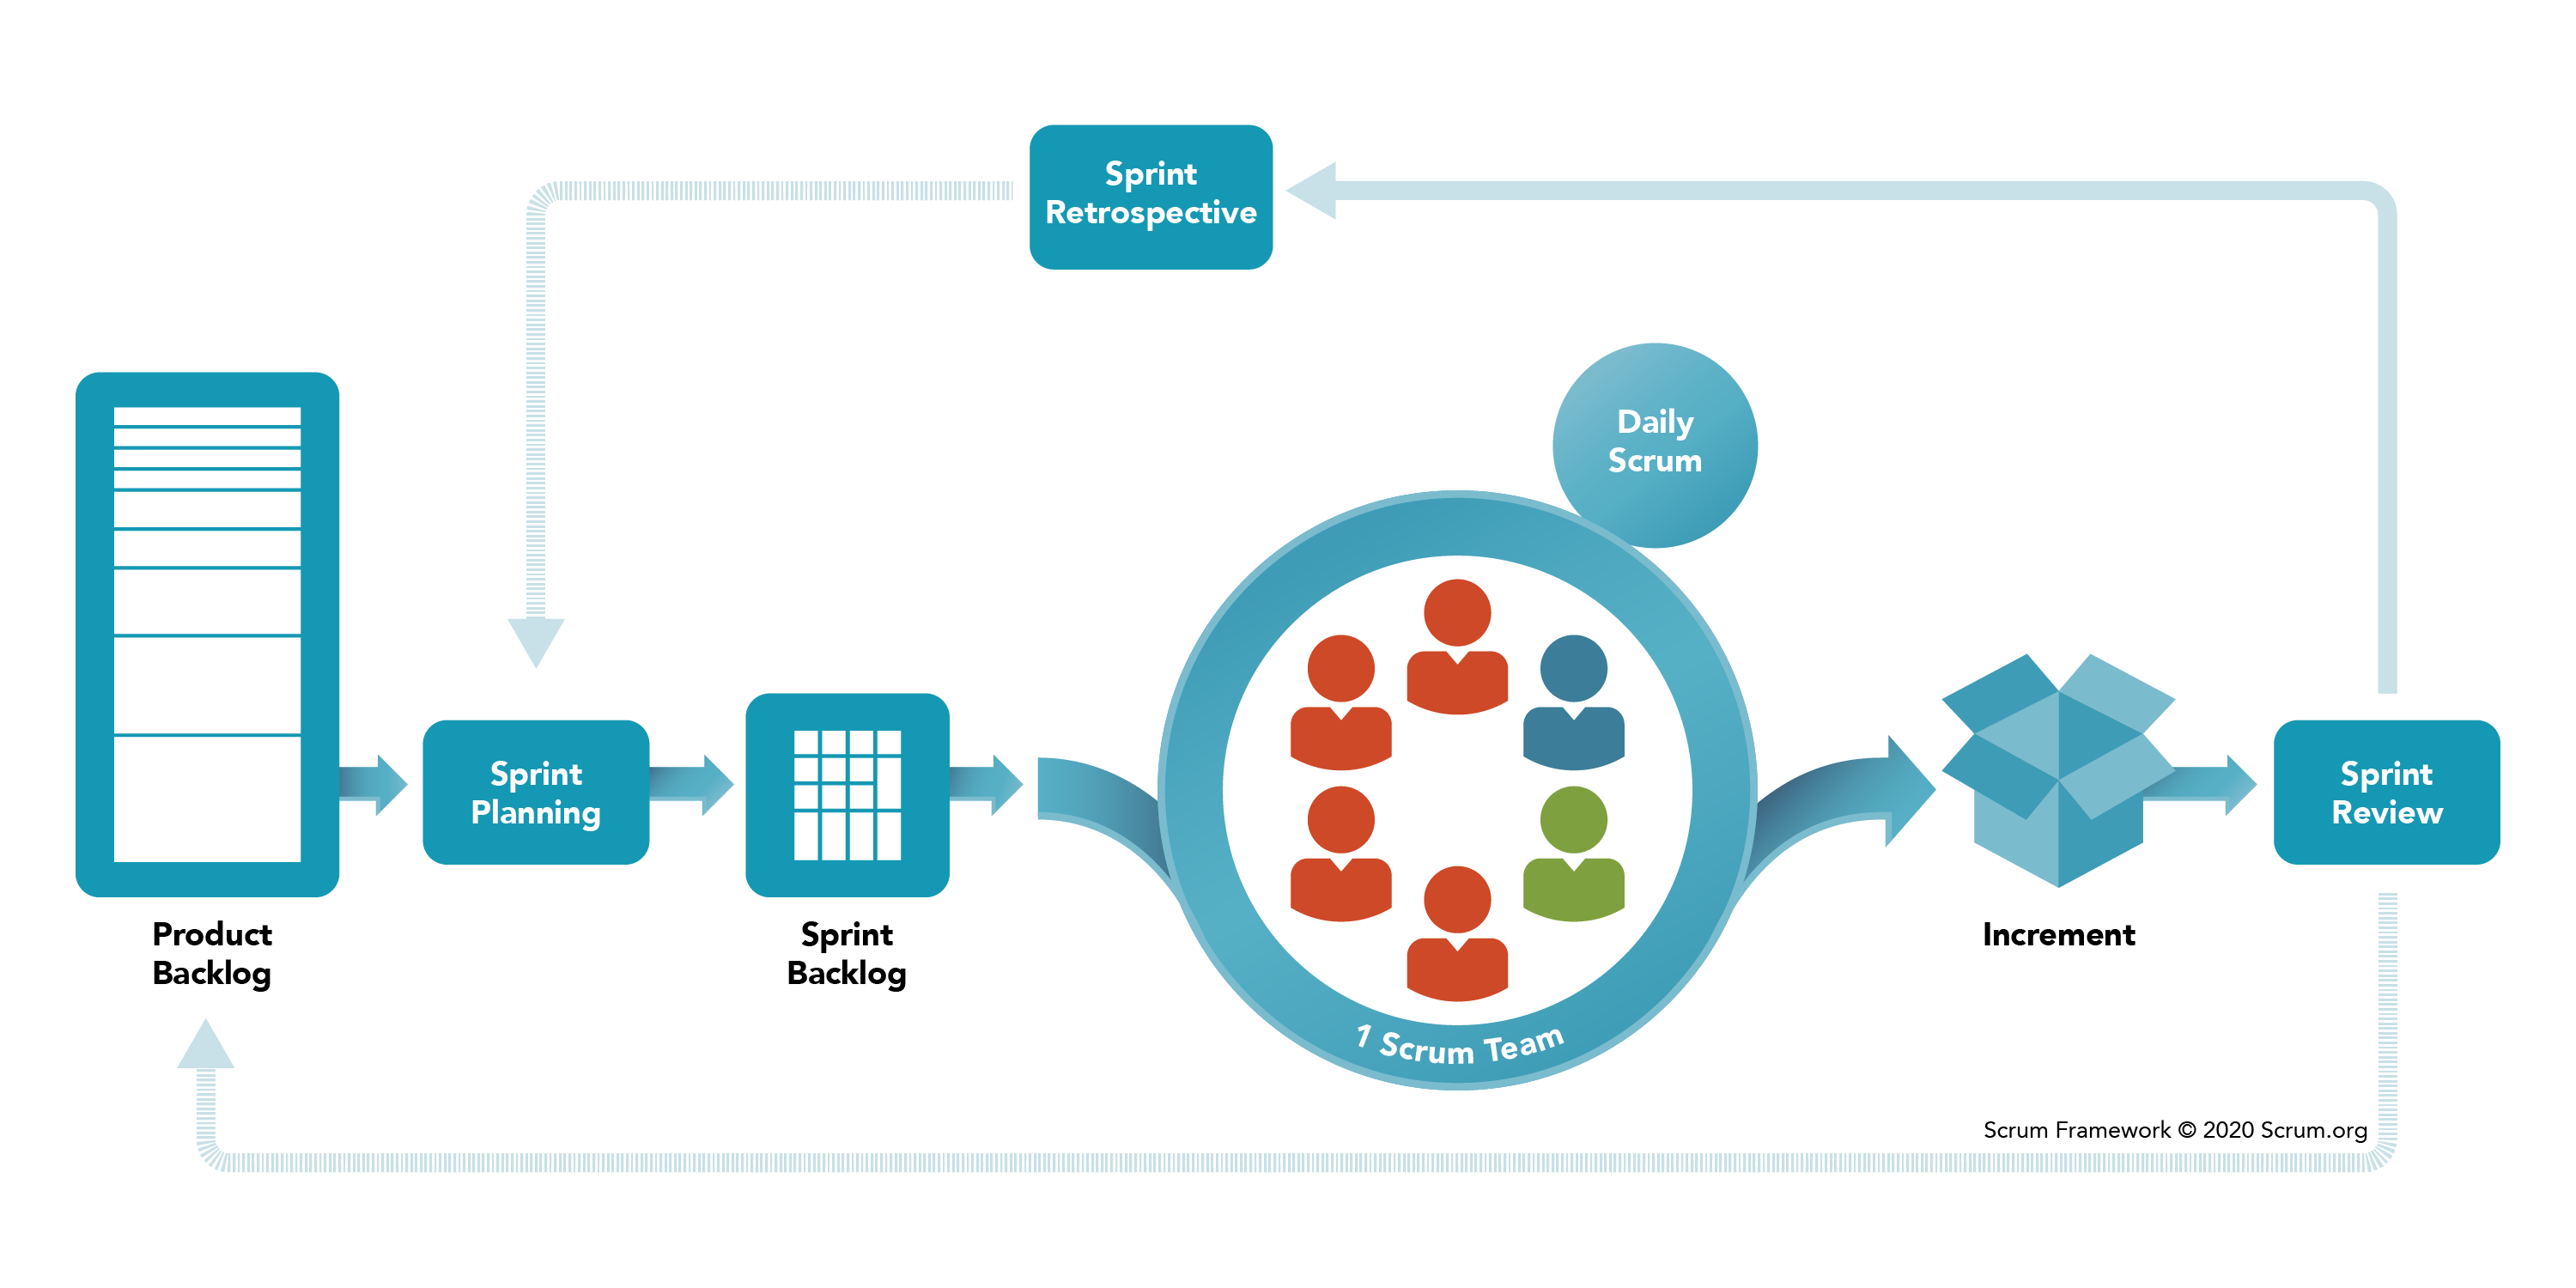
\includegraphics[width=1\textwidth]{img/chapter_4/scrum.png}
    \caption{Scrum framework}
\end{figure}
\noindent
Other than that, scrum master is assigned a role to the project manager who will be responsible for making a vision of final product of every sprint and present the project increment(result of each sprint) to supervisor and relay the feedback to scrum team.\\
Continous interaction between team and supervisor helps in proficient speed of development as well as quality software development indeed.Weekly meeting proved to be very effective to boost the productivity in team members and keep updated facts to supervisor.\\

\noindent
The use of iterative planning and feedback results in teams that can
continuously align a delivered product that reflects the invisioned product of a manager.
It easily adapts to changing requirements throughout the process by measuring
and evaluating the status of a project. The measuring and evaluating allows accurate and early visibility into the progress of the project. The ongoing change
can sometimes give both the client and the team more than they had originally
invisioned for the product. The Agile Method really is a winning solution for
everyone involved in software development.\\

\noindent
So, in the actual project development phase we tried to follow the above mentioned method as much as possible. Indeed we applied the scrum master and decided to conduct a weekly meeting with supervisor to present our progress and present our ideas to supervisor.\\

\noindent
Also, we tried to make a daily 15 mintues scrum meeting 8:45 to 9:00 AM in order to present and refresh on our working progress among each other.\\
We made a rule to have scrum implemented in a form below:-\\

\begin{table}
    \caption{Sprint Configuration}
    \centering
    \begin{tabular}{|l|l|}
        \hline
        \textbf{Sprint Length} & \textbf{2 weeks} \\
        \hline
        Story point weight & 1 story point = 1 hr \\
        \hline
        No.of working days per week & 4 days \\
        \hline
        No.of working hours per day & 3 hrs \\
        \hline
        No.of working days per sprint & 8 days \\
        \hline
        No.of working hours per sprint & 8*3 = 24 hrs \\
        \hline
    \end{tabular}\\
\end{table}

\noindent
We have altogether used 6 spaces inside our project workspace till now that are:-
\begin{enumerate}[label=\alph*.]
    \item Project plan
    \item wiki
    \item sprint - 1
    \item sprint - 2
    \item sprint - 3
    \item sprint - 4
\end{enumerate}
Then, for each of these sprint spaces we have made a list name as sprint backlog where we drag the ideas or tasks mentioned inside the project plan's backlog list. As per dscussion in our meeting each of the tasks are first created inside project plan's backlog.\\
As the tasks are assigned to team members one has to make an issue in related git repo project folder which then converts to the branch for working in technical way. Then, after all the commits are pushed into that branch then merge request is created for the project manager to check work in that branch then verify it finally to merge it with master branch.\\\\
Therefore in this procedure, whole ideation of problem solving broken down into small tasks and then conversion to git issues and finally branches relating to those issues merging with master is performed.\\ 

\section{Work division}
\subsection{Team member: Anusha Bajracharya}
\begin{enumerate}[label=\alph*.]
    \item Literature review on 3D model
          \begin{itemize}
              \item House-GAN: Relational Generative Adversarial Networks for Graph-constrained House Layout Generation
              \item Learning a Probabilistic Latent Space of Objects Shapes via 3D Generative Adversarial Modeling
              \item Learning Shape Priors for Single-View 3D Completion and Reconstruction
              \item Interactive 3D Modeling with a Generative Adversarial Network
              \item Plan2Scene: Converting Floorplans to 3D Scenes
              \item Raster-to-Vector: Revisiting Floorplan Transformation
          \end{itemize}
    \item 3D model representation
          \begin{itemize}
            \item Pixels, voxels, and views: A study of shape representations for single view 3D object shape prediction
          \end{itemize}
    \item{Familiarization with function}
          \begin{itemize}
              \item Activation function
          \end{itemize}
    \item{Familiarization with callback function}
          \begin{itemize}
              \item Checkpoints in Keras
          \end{itemize}
    \item GAN generator design
          \begin{itemize}
              \item U-net generator
              \item Double U-net generator
          \end{itemize}
\end{enumerate}
\subsection{Team member: Luja Shakya}
\begin{enumerate}[label=\alph*.]
    \item Literature review on architecture design
          \begin{itemize}
              \item U-Net: Convolutional Networks for Biomedical Image Segmentation
              \item DoubleU-Net: A Deep Convolutional Neural Network for Medical Image Segmentation
              \item Momentum Batch Normalization for Deep Learning with Small Batch Size
          \end{itemize}

    \item{Familiarization with callback function}
          \begin{itemize}
              \item Early stopping in Keras
          \end{itemize}
    \item{Diagram and tasks representation}
          \begin{itemize}
            \item TOP level structure diagram
            \item Ganttchart tasks estimation
          \end{itemize}
    \item{Generator metric}
          \begin{itemize}
            \item Inception score
            \item FID score
          \end{itemize}     
    \item{Mockup design}
          \begin{itemize}
          \item Spalsh screen
          \item Mainmenu
          \item Area selection
          \item Parcel to Footprint output screen
          \item Constraints addition
          \item Generated FP choose screen
          \item 3D render screen
          \end{itemize}
\end{enumerate}
\subsection{Team member: Niranjan Bekoju}
\begin{enumerate}[label=\alph*.]
    \item Literature review
\begin{itemize}
    \item Intelligent Home 3D: Automatic 3D-House Design from Linguistic Descriptions
    \item A U-Net Based Discriminator for GAN
    \item GAN Architecture Design
    \item The rendering equation
\end{itemize}
    \item Dataset preparation
\begin{itemize}
    \item Availability of the datasets using python script as zip file
\end{itemize}
\item{Familiarization with function}
\begin{itemize}
    \item Optimization function
\end{itemize}
\item{Familiarization with callback function}
\begin{itemize}
    \item TensorBoard in Keras
\end{itemize}
\item Architecture representation and preparation
\begin{itemize}
    \item Overall Architecture Design
    \item Base Image Creation
\end{itemize}
\item Architectural design
\begin{itemize}
    \item Custom Simple U-net + CNN
    \item Trainable Architecture
\end{itemize}
\item 3D model architecture
\begin{itemize}
    \item 3D model generation using segmented images
\end{itemize}
\end{enumerate}
\subsection{Team member: Sunil Banmala}
\begin{enumerate}[label=\alph*.]
\item Literature review
\begin{itemize}
    \item Transfer learning
\end{itemize}
\item Dataset preparation
\begin{itemize}
    \item Create principle/algorithm to generate the paired image
    \item Explore the currently available datasets
    \item Image processing using dilation and erode techniques
    \item Availability of the datasets using python script as zip file
\end{itemize}
\item Python script preparation
\begin{itemize}
    \item Parcel generation
    \item Parcel to footprint
    \item Footprint to room split
    \item Room split to furnished
\end{itemize}
\item{Familiarization with function}
\begin{itemize}
    \item Loss Function
\end{itemize}
\end{enumerate}

\section{Workload by status}
Among the tasks identified till now, 53.1\% of work is completed, 6.3\% of work is done but yet to be reviewed, 1.6\% of work is doing and 39.1\% of work is yet to be done which can be seen in the pie chart below generated automatically by the project management tool Clickup.
\begin{figure}[h]                 
    \centering                 
    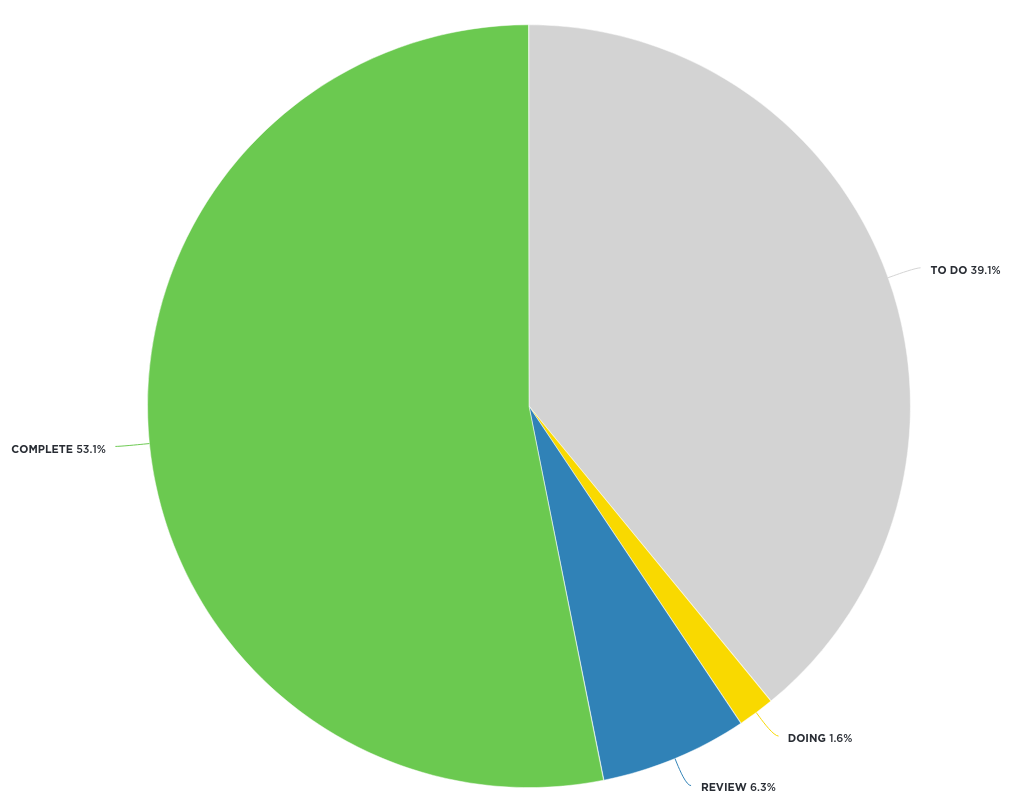
\includegraphics[width=.6\textwidth]{img/methodology/workload_by_status.png}               
    \caption{Progress of the project by status}                 
    \label{fig:workload-by-status}         
\end{figure}